\chapter{Tree Refinement}
\label{chap:tree}
% 0.5 Seiten

	With the existing capabilities of \ac{GCG} presented in the previous chapter, we continue with the main contributions of this thesis:
	
	\begin{itemize}
		\item A new module which is integrated into the detection framework of \ac{GCG} for reverse engineering semantic groupings of the original formulation.
		\item Additional auxiliary classifiers which implement constraint and variable classification based on information not currently used including examples of \textit{when} they are crucial detecting semantics.
	\end{itemize}

	This chapter is divided into three main section:
	
	\begin{enumerate}
		\item A short summary about the available information we have access to.
		\item What the motivation and goals are why and how we aim to process this information.
		\item The concrete algorithm and its most integral parts.
	\end{enumerate}
	
	Some concrete details about the implementation itself are not subject of the following sections, but are discussed in Chapter \ref{chap:impl}.

	\clearpage

	\section{Information}
	% 1 Seite
	
	\begin{figure}[ht!]
		\centering
		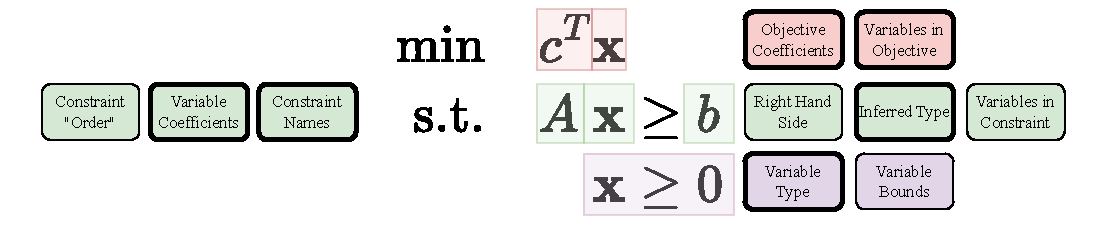
\includegraphics[scale=0.8]{Bilder/DrawIO/model_information}
		\caption{All parts of a model that contain useful information for semantic grouping of constraints and variables. Elements with a thick border are already used as a key concept in one of the existing detectors.}
		\label{fig:tree:information}
	\end{figure}
	
	Before we present any algorithmic details, we give an overview about the available information.
	
	\begin{enumerate}
		\item \textbf{Objective}: For the objective functions, information about the participating variables and their coefficients is available. For some models e.g. for Bin-Packing, this information alone is sufficient to partition the variables.
		\item \textbf{Coefficients}:
		The use of coefficients to classify constraints and variables was already in discussed in Section \ref{chap:gcg:classifiers}.
		\item \textbf{Bounds}: For all variables $lb \leq x \leq ub$ information about their lower- and upper-bounds is available.
		Furthermore, the left- and right-hand-side of linear constraints $lhs \leq \sum_i a_i x_i \leq rhs$ are available as well.
		\item \textbf{Types}: Variable types such as \textit{Integer} are usually stated explicitly in the input format. If not, then information about the variable bounds can be used to deduce a type, e.g. $0 \leq x \leq 1$ is a strong indicator that $x$ is a \textit{Binary} variable.
		\item \textbf{Names}: If specified by the modeler, then variables and constraints might have meaningful names which can be used as a strong indicator which constraints and variables belong to the same group.
		\item \textbf{Order}: In contrast to other kinds of information, the constraint \enquote{order} is no intrinsic property of the model itself. With the term \enquote{order}, we refer to the order of the constraints as specified in the input format. When a model is created e.g. via. a script, constraints are usually added in \textit{blocks} by the modeler. This information is used in Section \ref{chap:tree:classifiers:voting} to conceptualize a classifier based on that.
	\end{enumerate}
	
	\section{Motivation}
	% 2 Seiten
	
	\section{Classifiers}
	% 2 Seite
	
		\subsection{Bounds}
		
			
		
		\subsection{Relaxed MIPLIB types}
			
		\subsection{Ordered Voting}
		\label{chap:tree:classifiers:voting}
		
%	\section{Tree Refinement}
%	% 4 Seiten
%	
%		\begin{figure}[ht!]
%			\centering
%			\includesvg{Bilder/Hierarchy/hierarchy_binpack_NOP}
%			\caption{Test}
%			\label{fig:tree:binpackNOP}
%		\end{figure}
		
	\section{Strategies}
	
		
	
		\subsection{Slice}
		
		\subsection{Fast}
		
		\subsection{Recursive}
		
	\section{Rules}
	
		
	
	\section{Scoring}
	% 1 Seite

		\subsection{Rand Score}
		% 1 Seite

		\subsection{Connected Block Score}
		% 1 Seite
